\section{Implementation}
Lorem ipsum

\subsection{Architecture}

\subsubsection{Data Structures}

\paragraph{WAV File Wrapper}
For conveniently accessing the data contained in the wave file, we created the WaveFileWrapper class.

\paragraph{Filter Results}
The filter will return its findings as an object of the FilterResult class. This data class contains all information from the audio file that is need for rendering the report. 

\begin{itemize}
    \item duration: the length of the recording in seconds
    \item durationOverLimit: the total amount of time in seconds for which the threshold was exceeded
    \item peak: the peak RMS in dB(A)
    \item average: the average RMS in dB(A)
    \item samplesOverLimit: a list of all samples which exceeded the threshold
\end{itemize}


The class Sample represents a RMS sample which exceeded the threshold. 

\begin{itemize}
    \item time: seconds since the beginning of the recording. As the RMS is used for analyzing, the time represents the average time of all samples used for calculating it.
    \item decibel: the RMS dB(A) of that point in time
\end{itemize}

\begin{figure}[H]
    \centering
    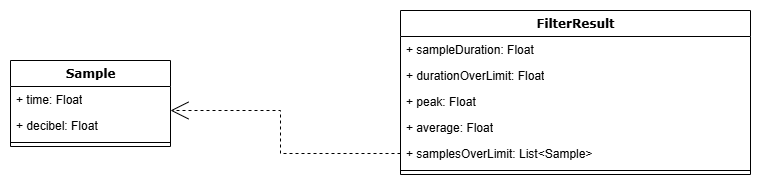
\includegraphics[width=0.8\textwidth]{../assets/interface.png}
    \caption{Sqeuence diagram of steps involved when creating a noise report}
\end{figure}

\subsection{Processes}
The following diagram shows which steps are involved when creating a noise report from a wave file.

\begin{figure}[H]
    \centering
    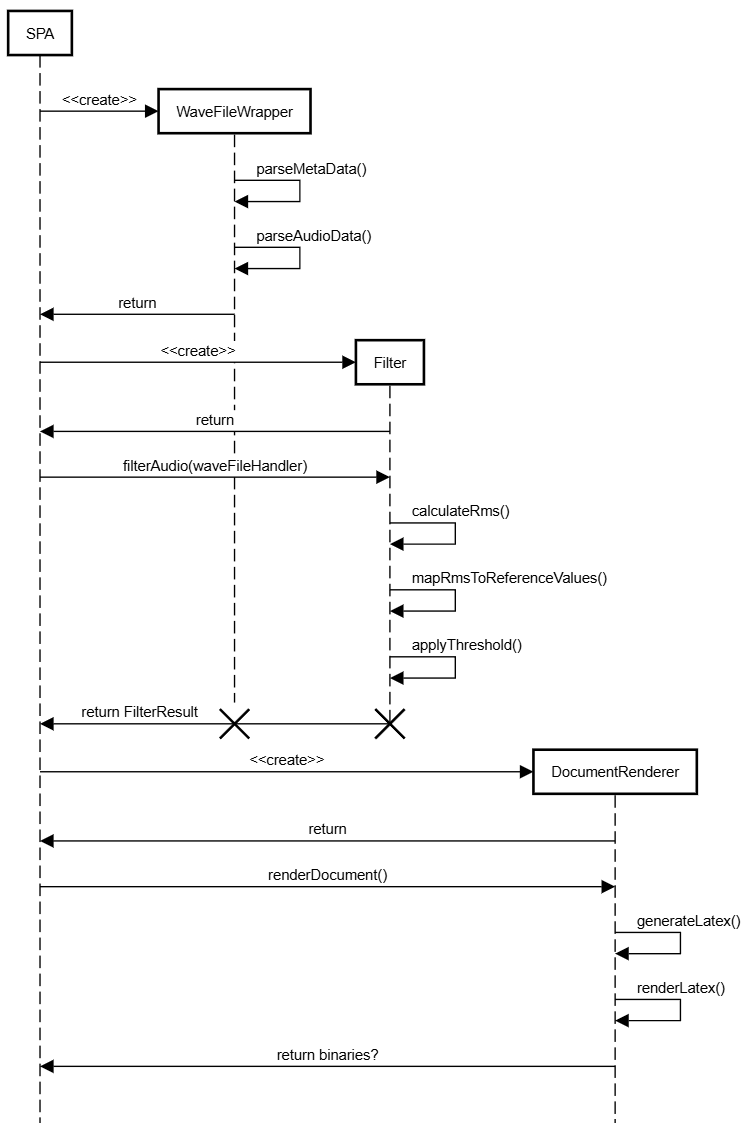
\includegraphics[width=0.8\textwidth]{../assets/sequence_diagram_from_wave_file_to_pdf.png}
    \caption{Sqeuence diagram of steps involved when creating a noise report}
\end{figure}

\subsubsection{Parsing the Wave File}
The WaveFileWrapper class will be responsible for parsing the file. The format itself is straight forward\cite{wav_file_format_wikipedia}, the only importend thing is that the whole file is Little-Endian. It starts with a 12 byte header which we use to verify that the given file is actually a wave file. After the header comes a 24 byte block which contains information about the data format. We are interested in the following fields:
\begin{itemize}
    \item FormatBlocID (4 bytes): is used to verfy that it is a known format. This field should always have the value 'fmt '.
    \item BlocSize (4 bytes): is needed to parse the format information itself 
    \item AudioFormat (2 bytes): only handle PCM i guess?
    \item NbrChannels (2 bytes): is used to parse individual samples
    \item Frequence (4 bytes): number of samples per second, this is needed for filtering and summarzing 
    \item BitsPerSample (2 bytes): number of bits for a single sample for a single channel, is used to parse individual samples
\end{itemize}
After the format block comes the data block. This block starts with a 4 byte long DataBlocID, which should always have the value 'data'. The next 4 byte represent the number of samples in the data. After that comes the actual audio data. To parse a single sample, we need to parse a frame. A frame contains the data of all channels and has therefore a size of \[\frac{NbrChannels * BitsPerSample}{8}\] bytes. 

\subsubsection{Calculating Decibel Values}
If an audio file consists of several channels, we use the average of the channels as the value of the sample.
When we want to analyse where a certain decibel threshold has been exceeded, we must have accurate values. People only perceive something as loud if it is loud over a longer period of time. Short peaks are perceived less. Therefore, when determining the effective loudness of audio, we do not use the loudness of individual samples, but rather the average of a number of samples over a certain period of time. We will, as usual when working with audio, use the root mean squere (RMS), as we are interested in the absolute amplitude values.
The calculated average then depends heavily on how long the time period is. In practice, 300ms is usually used\cite{timespan_for_audio_rms_calculate}. This is also the default value, which can be adjusted by the user via the settings.
The decibel value is calculate with the following formula\cite{decibel_wikipedia}:
\[20 * \log_{10} (sample)\] 

As mentioned in the introduction, the audio file only contains relativ values. We therefore need to map the RMS values to the number range of the reference values, where the smallest sample is mapped to the minimal dB(A) and the largest sample is mapped to the maximal dB(A) measured. 
